\chapter{Construction of \CY's}
\label{sec:constructions}

Let $E_6$ be the hexagon as a simplicial complex. We form the associated Stanley--Reisner scheme $\P(E_6)$. It is a degenerated elliptic curve in $\P^5$.

\begin{lemma}
The Hilbert polynomial of $\P(E_6)$ is $h(t)=6t$.
\end{lemma}
\begin{proof}
We want to count the dimension of $S_t=S_{E_6}(t)$. Any monomial in $S_k$ has support on the simplicial complex $E_6$, so its support is either a vertex or an edge. In the first case, the monomial has the form $x_i^t$, so there are six of these.

In the other case, it has the form $x_i^ax_{i+1}^b$, with $a+b=t$ and $a,b \neq 0$. Counting, there are $6(t-1)$ of these monomials. In total, the dimension is $6+6(t-1)=6t$.
\end{proof}
\begin{remark}
Alternatively, we could note that $\P(E_6)$ smooths to an elliptic curve of degree $6$. Since Hilbert polynomials are constant in flat families, it follows from Riemann--Roch that $h(t)=\deg \OO_{\P(E_6)}(t)-1+1=6t$.
\end{remark}

Note that the Hilbert polynomial only differ from the Hilbert function for $t=0$. Let $\K$ be the simplicial complex $E_6 \ast E_6$. It is a triangulation of the 3-sphere.

\begin{lemma}
The Hilbert polynomial of $\P(\K)$ is $h(t)=6t^3+6$.
\end{lemma}
\begin{proof}
The homogeneous coordinate ring $S=\oplus_{t \geq 0} S_t$ of $\P(\K)$ is the twofold tensor product of $\P(E_6)$. It follows from the previous lemma that
\[
\dim S_t = \sum_{i+j=k, ij \neq 0} 36ij + 12k,
\]
where the last term is a correction term because $h(t) \neq 1$. It is now a routine computation using formulas for sums of squares to verify the claim.
\end{proof}

It is the deformations of $\P(\K)$ that we will study in this thesis. \todo{Something about choosing another triangulation, making T2 smaller}

\section{Toric deformations}

\begin{figure}
\centering
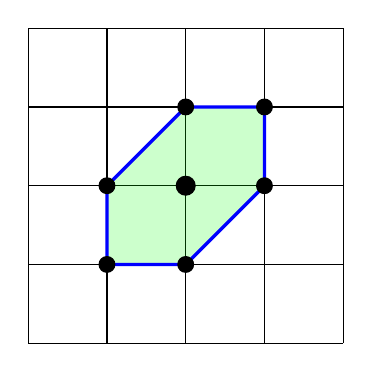
\begin{tikzpicture}
  \draw (0, 0) grid (4, 4);  
\draw [very thick, color=blue, fill=green, fill opacity=0.2]
(1,1) -- (2,1) -- (3,2) -- (3,3) -- (2,3) -- (1,2) -- cycle;
\draw [fill=black]  (1, 1) circle (0.1);
\draw [fill=black]  (2, 1) circle (0.1);
\draw [fill=black]  (3, 2) circle (0.1);
\draw [fill=black]  (3, 3) circle (0.1);s
\draw [fill=black]  (2, 3) circle (0.1);
\draw [fill=black]  (1, 2) circle (0.1);
\draw [fill=black]  (2, 2) circle (0.12);
\end{tikzpicture}
\caption{A hexagon.}
\label{fig:hexagon}
\end{figure}

By starring $E_6$ with a vertex, we get a triangulation of the disk. Denote by $\nabla$, the hexagon in  \cref{fig:hexagon}. By Theorem 8.3 and Corollary 8.9 in \cite{sturmfels}, there is a one-one correspondence between unimodular regular triangulations of $\nabla$ and the square-free initial ideals of the toric ideal of $\P(\nabla)$. 

This means that $E_6 \ast \{ pt \}$ smooths to the del Pezzo surface of degree $6$, and also that $\P(E_6)$ smooths to an anticanonical section of $\dP6$. 

\todo{Talk about the join of two del pezzos}

$X_0$.

\section[Smoothings of X0]{Smoothings of $X_0$}

We will exploit the fact that the cone over $\dP6$ have two smoothings two produce two smoothings of $X_0$.

\subsection{The first construction}

Let $E$ be a 3-dimensional vector space. Let $\{e_1,e_2,e_3\}$ be a basis for $E$. Then $S_3$ act on $E$ by $e_i \mapsto e_{\sigma(i)}$. It also act on $(E \otimes E)^{\oplus 2}\simeq k^{18}$. There is a $\Z_2$-action switching the factors. Let $\P=\P(k^{18})$. Then $S_3 \times \Z_2\simeq D_6$ act on $\P$. 

The elements of $\P^{17}$ are pairs of $3 \times 3$-matrices, not both zero. Let $M$ be the closure of the set of pairs $(A,B)$ where $\rank A = \rank B = 1$. 

If $\P^{17}$ have coordinates $x_1,\ldots,x_{18}$, let $M_1, M_2$ be generic matrices:
\[
M_1 = \begin{pmatrix}
x_1 & x_2 & x_3 \\
x_4 & x_5 & x_6 \\
x_7 & x_8 & x_9 
\end{pmatrix}\,
\text{ and }
M_1 = \begin{pmatrix}
x_{10} & x_{11} & x_{12} \\
x_{13} & x_{14} & x_{15} \\
x_{16} & x_{16} & x_{17}
\end{pmatrix}.
\]

Then $M$ is defined by the zeroes of the $2 \times 2$-minors of $M_1$ and $M_2$. Note that $M$ is the projective join of two copies of $\mathbb P^2 \times \mathbb P^2 \hookrightarrow \mathbb P^8$. 

The variety $M$ is $9$-dimensional: the affine cone over $M$, $C(M)$, is equal to $C(\mathbb P^2 \times \P^2) \times C(\mathbb P^2 \times \P^2)$. This variety has dimension $5+5=10$, hence its projectivization $M$ is $9$-dimensional. 

The singular locus of $M$ consists of the pairs $(0,B)$, and $(A,0)$, where $\rank A= \rank B = 1$, hence $\dim \sing M = 4$. By Bertini's theorem, intersecting $M$ with a codimension $6$ hyperplane gives a smooth variety $X_1$.

Note that by putting $x_1=x_5=x_6$ and $x_{10}=x_{14}=x_{17}$, we get the join of two del Pezzos, so we see that $X_1$ deforms to $X_0$ \todo{consistent notation}. It follows that $X_1$ is a smooth Calabi-Yau.

\begin{proposition}
\label{prop:x1euler}
$X_1$ has topological Euler characteristic $-72$. 
\end{proposition}
\begin{proof}
This is a computation in \MM. Since computing the whole cotangent sheaf of $X_1$ is impossible with current computer technology, we make use of standard exact sequences. Let $\mathscr I$ be the ideal sheaf of $M$ in $\P^{17}$. First off, we have the exact sequence
$$
0 \to \restr{\mathscr I/\mathscr I^2}{X} \to \restr{\Omega_\P^1}{X} \to \restr{\Omega_M^1}{X} \to 0.
$$
The \MM command \texttt{eulers} computes the Euler characteristics of generic linear sections of a sheaf $\mathscr F$. Using this command, we find that $\chi(\restr{\mathscr I/\mathscr I^2}{X})=-180$. Using the exact sequence
$$
0 \to \restr{\Omega_\P^1}{X} \to \OO_X(-1)^{18} \to \OO_X \to 0,
$$
we find that the Euler characteristic of $\restr{\Omega_\P^1}{X}$ is $-216=12\cdot 18$. It follows from the first exact sequence that $\restr{\Omega_M^1}{X}$ has Euler characteristic $-36$.

Since $X$ is a complete intersection, the conormal sequence looks like
$$
0 \to \OO_X(-1)^6 \to \restr{\Omega_M}{X}  \to \Omega_X^1 \to 0.
$$
Hence $\chi(\Omega_X^1) = -36+72 = 36$.

It follows that the topological Euler characteristic is $\chi_X = -2\chi(\Omega_X^1)=-72$.
\end{proof}

\subsection{The second construction}

Let $E$ be a $2$-dimensional vector space with basis $\{e_1,e_2\}$. Let $\P=\P\left((E \otimes E \otimes E)^{\oplus 2}\right)$. Then $\P=\P^{15}$. There is an action of $S_3$ on $E \otimes E \otimes E$ given by permuting the tensor factors. Combining this with a $\Z_2$ switching $A$ and $B$, we get a $S_3 \times \Z \simeq D_6$-action on $\P$. 

The elements of $\P$ are pairs $(A,B)$ of $2 \times 2 \times 2$-tensors, not both zero. 

Let $N$ be the closure of set of pairs $(A,B)$ where both $A$ and $B$ have tensor rank $1$\footnote{An element of $E^\otimes 3$ have rank $1$ if it is a pure tensor. It has rank $k$ if it can be written as a sum of $k$ pure tensors.}. A pure $2 \times 2 \times 2$-tensor can be visualized as a box in $\Z^3$ of unit volume. Let the variables on $\P$ be $a_{ijk}$ and $b_{ijk}$ for $i,j,k=0,1$. See the diagram in \vref{fig:222tensor}.

\begin{figure}
\centering
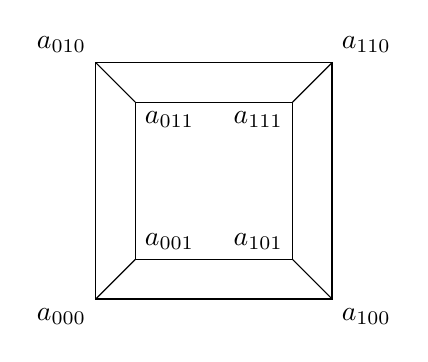
\begin{tikzpicture}
\draw (0,0) -- (3,0) -- (3,3) -- (0,3) -- cycle;
\draw (0.5,0.5) -- (2.5,0.5) -- (2.5,2.5) -- (0.5,2.5) -- cycle;
\draw (0,0) -- (0.5,0.5);
\draw (3,0) -- (2.5,0.5);
\draw (3,3) -- (2.5,2.5);
\draw (0,3) -- (0.5,2.5);
\node[below left] at (0,0) {$a_{000}$};
\node[below right] at (3,0) {$a_{100}$};
\node[above right] at (3,3) {$a_{110}$};
\node[above left] at (0,3) {$a_{010}$};

\node[above right] at (0.5,0.5) {$a_{001}$};
\node[above left] at (2.5,0.5) {$a_{101}$};
\node[below left] at (2.5,2.5) {$a_{111}$};
\node[below right] at (0.5,2.5) {$a_{011}$};
\end{tikzpicture}
\caption{A $2 \times 2 \times 2$-tensor.}
\label{fig:222tensor}
\end{figure}

The equations of the set of rank $1$ tensors are obtained as the ''minors'' along the $6$ sides together with the minors along the $4$ long diagonals, giving a total of $9$ binomial equations. 

Note that $N$ is the projective join of two copies of $\P^1 \times \P^1 \times \P^1$.

The singular locus of $N$ consists of the pairs $(A,0)$ and $(0,B)$ where both $A,B$ have rank $1$. Hence the singular locus is of dimension $3$.

Intersecting $N$ with a codimension $4$-hyperplane gives a smooth variety $X_2$. It is Calabi-Yau and has topological Euler characteristic $-48$.

\begin{proposition}
The topological Euler characteristic of $X_2$ is $-48$.
\end{proposition}
\begin{proof}
The proof is identical to the proof of \cref{prop:x1euler}.
\end{proof}
